\chapter{Champs faibles, ondes gravitationnelles et principe de l’action}

Les équations exactes de la relativité générale sont non linéaires, et leur expression en composantes peut devenir redoutable avant même qu’on ait résolu un seul problème physique. Pour cette dernière leçon du cours, mieux vaut distinguer les principes des calculs. Nous examinerons ce que deviennent les équations d’Einstein lorsque le champ gravitationnel est faible, nous identifierons les ondes que contient cette approximation, puis nous verrons comment les équations complètes du champ s’inscrivent dans un principe d’action remarquablement compact.

Trois questions structurent la discussion. Que signifie un champ gravitationnel faible ? Pourquoi la théorie faible est-elle linéaire alors que la théorie exacte ne l’est pas ? Et quels effets physiques permettent de distinguer une onde gravitationnelle d’une simple ondulation des coordonnées ?

\section{Petite perturbation d’une géométrie d’équilibre}

La faiblesse est une méthode d’approximation. Si une perturbation sans dimension est de l’ordre de \(\epsilon\ll1\), son carré est de l’ordre de \(\epsilon^2\), et un calcul au premier ordre néglige systématiquement ce dernier terme. L’exemple classique est celui d’un système mécanique qui effectue de petites oscillations autour de l’équilibre. Ses équations exactes peuvent être non linéaires, mais des oscillations suffisamment petites obéissent à des équations linéaires.

En gravitation, l’état d’équilibre sera l’espace-temps plat et vide. Partons de l’équation du vide d’Einstein,
\begin{equation}
 R_{\mu\nu}-\frac12 g_{\mu\nu}R=0.
 \label{eq:l10-vacuum-einstein}
\end{equation}
Sa trace en quatre dimensions donne
\begin{equation}
 g^{\mu\nu}
 \left(R_{\mu\nu}-\frac12 g_{\mu\nu}R\right)
 =R-2R=-R=0,
\end{equation}
L’équation du vide est donc équivalente à
\begin{equation}
 R_{\mu\nu}=0.
 \label{eq:l10-ricci-flat}
\end{equation}

\begin{figure}[htbp]
\centering
\includegraphics[width=0.68\textwidth]{lecture_10_figure_02.png}
\caption{L’équation du vide \(R_{\mu\nu}=0\), isolée au début de l’argument sur les champs faibles.}
\lectureframe{00:03:11}
\end{figure}

Ici, l’équilibre désigne une solution sans source et indépendante du temps. L’espace-temps plat est la solution de ce type la plus simple. Une précision est essentielle : la platitude ne signifie pas que les composantes de la métrique soient égales à une matrice particulière dans tout système de coordonnées. Elle signifie qu’on peut choisir des coordonnées inertielles dans lesquelles
\begin{equation}
 g_{\mu\nu}=\eta_{\mu\nu}.
\end{equation}
Cette distinction entre une géométrie et les coordonnées qui servent à la décrire deviendra bientôt la subtilité centrale.

Imaginons maintenant une source violente, telle qu’un système binaire compact. Son champ proche peut être intense, mais loin de la source, la perturbation se propage et devient petite. Dans un système de coordonnées adapté, la métrique peut alors s’écrire
\begin{equation}
 g_{\mu\nu}(x)=\eta_{\mu\nu}+h_{\mu\nu}(x),
 \qquad |h_{\mu\nu}|\ll1.
 \label{eq:weak-split}
\end{equation}
La perturbation \(h_{\mu\nu}\) peut dépendre des quatre coordonnées de l’espace-temps. La faiblesse signifie que l’on néglige les termes d’ordre supérieur au premier.

\section{Ce qui subsiste au premier ordre}

Le tenseur de Ricci complet est trop long pour être utile à ce stade. Sa structure suffit. Les symboles de Christoffel contiennent la métrique inverse et une dérivée de la métrique, tandis que la courbure contient une dérivée d’un symbole de Christoffel et un produit de deux symboles de Christoffel :
\begin{equation}
 \Gamma\sim\frac12 g^{-1}\partial g,
 \qquad
 R\sim\partial\Gamma+\Gamma\Gamma.
 \label{eq:curvature-skeleton}
\end{equation}

\begin{figure}[htbp]
\centering
\includegraphics[width=0.84\textwidth]{lecture_10_figure_03.png}
\caption{La décomposition en champ faible et la construction schématique
\(R\sim\partial\Gamma+\Gamma\Gamma\). La notation fait apparaître les ordres en
\(h\) sans développer chaque indice.}
\lectureframe{00:10:17}
\end{figure}

La métrique inverse se déduit de
\(g^{\mu\alpha}g_{\alpha\nu}=\delta^\mu{}_\nu\). Au premier ordre,
\begin{equation}
 g^{\mu\nu}=\eta^{\mu\nu}-h^{\mu\nu}+O(h^2),
 \label{eq:inverse-weak}
\end{equation}
où les indices de \(h\) sont relevés à l’aide de la métrique de fond. Dans des coordonnées inertielles, la métrique de fond est constante,
\begin{equation}
 \partial_\alpha\eta_{\mu\nu}=0,
\end{equation}
et par conséquent
\begin{equation}
 \partial_\alpha g_{\mu\nu}
 =\partial_\alpha h_{\mu\nu}.
\end{equation}
On obtient donc
\begin{equation}
\begin{aligned}
 \Gamma&=O(\partial h),\\
 R_{\mu\nu}
 &=O(\partial\partial h)+O\bigl((\partial h)^2\bigr)\\
 &\quad+O(h\,\partial\partial h).
\end{aligned}
 \label{eq:ricci-orders}
\end{equation}

\begin{figure}[htbp]
\centering
\includegraphics[width=0.84\textwidth]{lecture_10_figure_04.png}
\caption{Le développement de la métrique inverse au tableau et l’observation que
\(\partial\eta=0\). Seules les dérivées de \(h_{\mu\nu}\) subsistent au premier ordre.}
\lectureframe{00:11:55}
\end{figure}

Les deux derniers termes de l’équation~\eqref{eq:ricci-orders} sont quadratiques en la perturbation et sont omis. Les équations du vide sont donc des équations linéaires faisant intervenir les dérivées secondes de \(h_{\mu\nu}\). C’est tout ce que signifie la linéarisation. Cela ne signifie pas que la théorie exacte d’Einstein soit linéaire.

\begin{classroomqa}
\audiencequestion{Le tenseur de courbure a quatre indices, tandis que le tenseur de Ricci en a deux. Si deux dérivées portent déjà des indices et que \(h_{\mu\nu}\) en porte deux autres, comment s’effectue le comptage des indices ?}
\lecturerresponse{On obtient le tenseur de Ricci en contractant une paire d’indices du tenseur de courbure. La métrique utilisée pour cette contraction laisse deux indices libres, précisément ceux de \(R_{\mu\nu}\). La forme symbolique \(\partial\partial h\) ne fait pas apparaître ces contractions : elle indique l’ordre des termes, et non une formule complète avec indices.
\lecturetimestamp{00:18:45--00:19:53}}
\end{classroomqa}

\begin{classroomqa}
\audiencequestion{La contraction avec la métrique inverse introduit-elle des termes tels que \(h\,\partial^2h\), et si oui, pourquoi peut-on les négliger ?}
\lecturerresponse{C’est le cas. En remplaçant \(g^{-1}\) par
\(\eta^{-1}-h+\cdots\), on obtient le terme linéaire
\(\eta^{-1}\partial^2h\) ainsi que des corrections contenant une deuxième puissance de \(h\). Ces dernières sont quadratiques. La même règle permet d’écarter
\(h\,\partial h\), \(h\,\partial^2h\) et
\((\partial h)^2\). Ne conserver qu’une seule puissance de la perturbation, c’est précisément faire l’approximation considérée.
\lecturetimestamp{00:19:55--00:21:14}}
\end{classroomqa}

\section{Pourquoi les équations prennent la forme d’ondes}

Des équations de champ faisant intervenir des dérivées secondes suggèrent naturellement une propagation ondulatoire. Pour une fonction scalaire se propageant selon l’axe \(z\), l’équation type est
\begin{equation}
 \left(\partial_t^2-\partial_z^2\right)\phi=0,
\end{equation}
dont les solutions comprennent des profils arbitraires se propageant vers la droite ou vers la gauche,
\begin{equation}
 \phi(z,t)=f(z-t)+g(z+t).
\end{equation}
En trois dimensions d’espace, la même équation s’écrit
\begin{equation}
 \left(\partial_t^2-\nabla^2\right)\phi=0.
\end{equation}
Sa linéarité autorise la superposition : la somme de deux solutions est encore une solution.

La gravitation n’est pas un champ scalaire. La perturbation possède des composantes tensorielles, et l’équation \(R_{\mu\nu}=0\) semble d’abord fournir de nombreuses équations pour ces composantes. Elles ne sont pas toutes indépendantes : certaines sont des contraintes, d’autres traduisent la liberté de choix des coordonnées. L’analogie est celle de la théorie de Maxwell, où un ensemble d’équations de champ ne laisse finalement subsister que les ondes transversales physiques.

Une fois imposées des conditions de coordonnées adaptées, les composantes radiatives obéissent à une équation d’onde ordinaire,
\begin{equation}
 \Box h_{\mu\nu}=0,
 \qquad
 \Box=\eta^{\alpha\beta}\partial_\alpha\partial_\beta.
 \label{eq:linear-wave}
\end{equation}
Les signes précis dans \(\Box\) dépendent de la convention de signature ; le contenu, lui, ne change pas. Les perturbations se propagent sur le cône de lumière.

\section{Les ondulations des coordonnées ne sont pas des ondes gravitationnelles}

Avant de considérer toute solution des équations linéarisées comme une onde physique, revenons à la réserve concernant les coordonnées. On peut décrire l’espace plat avec des lignes de coordonnées courbes. Les composantes de la métrique diffèrent alors de leurs valeurs cartésiennes, même si la courbure reste nulle.

Le tableau lui-même en fournit un exemple. Traçons des coordonnées cartésiennes sur sa surface plane et écrivons
\begin{equation}
 ds^2=\delta_{mn}\,dx'^m dx'^n.
\end{equation}
Puis attribuons aux mêmes points des coordonnées légèrement ondulées,
\begin{equation}
 x'^m=x^m+f^m(x).
 \label{eq:small-coordinate-change}
\end{equation}
Les différentielles deviennent
\begin{equation}
 dx'^m=dx^m+\partial_n f^m\,dx^n.
\end{equation}
En substituant ces expressions dans l’élément de ligne et en ne conservant que le premier ordre en \(f\), on obtient
\begin{align}
 ds^2
 &=\delta_{mn}dx^m dx^n\\
 &\quad+\left(\partial_m f_n+\partial_n f_m\right)dx^m dx^n
 +O(f^2).
\end{align}
Ainsi, une perturbation apparente de la forme
\begin{equation}
 h_{mn}=\partial_m f_n+\partial_n f_m
 \label{eq:pure-gauge}
\end{equation}
peut ne décrire aucune nouvelle géométrie. Il s’agit de l’espace plat en coordonnées ondulées.

\begin{figure}[htbp]
\centering
\includegraphics[width=0.84\textwidth]{lecture_10_figure_05.png}
\caption{Le calcul des ondulations de coordonnées au tableau. Un léger changement de coordonnées induit un \(h_{mn}\) d’apparence faible, même si la surface du tableau reste plate.}
\lectureframe{00:27:54}
\end{figure}

L’équation~\eqref{eq:pure-gauge} est la forme linéarisée de la liberté de choix des coordonnées, ou liberté de jauge. Il faut imposer des conditions supplémentaires pour éliminer ces fausses perturbations. L’algèbre détaillée de la jauge n’est pas développée ici. Son rôle est toutefois essentiel : elle élimine les changements de description tout en préservant les changements de courbure. Une fois prises en compte la liberté de choix des coordonnées et les équations de contrainte, le contenu physique se réduit à deux polarisations indépendantes de l’onde.

\begin{figure}[htbp]
\centering
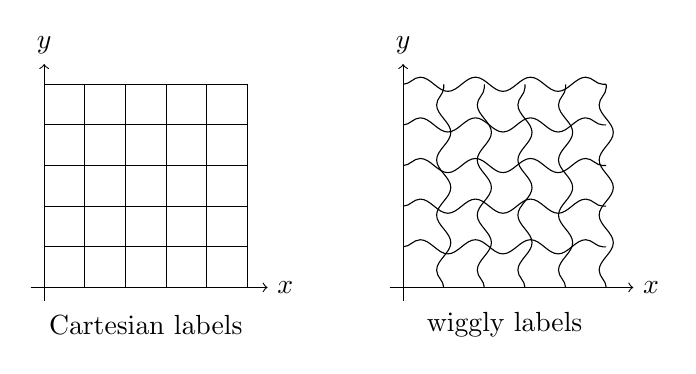
\begin{tikzpicture}[scale=0.86]
\begin{scope}
\draw[->] (-0.2,0) -- (3.3,0) node[right] {$x$};
\draw[->] (0,-0.2) -- (0,3.3) node[above] {$y$};
\foreach \u in {0.6,1.2,1.8,2.4,3.0}{
  \draw (\u,0) -- (\u,3.0);
  \draw (0,\u) -- (3.0,\u);
}
\node at (1.5,-0.55) {Cartesian labels};
\end{scope}
\begin{scope}[xshift=5.3cm]
\draw[->] (-0.2,0) -- (3.4,0) node[right] {$x$};
\draw[->] (0,-0.2) -- (0,3.3) node[above] {$y$};
\foreach \u in {0.6,1.2,1.8,2.4,3.0}{
  \draw[decorate,decoration={snake,amplitude=0.09cm,segment length=0.7cm}]
    (\u,0) -- (\u,3.0);
  \draw[decorate,decoration={snake,amplitude=0.09cm,segment length=0.7cm}]
    (0,\u) -- (3.0,\u);
}
\node at (1.5,-0.55) {wiggly labels};
\end{scope}
\end{tikzpicture}
\caption{La géométrie reste plate tandis que le réseau de coordonnées change. Les seules composantes de la métrique ne permettent pas de décider si une perturbation est physique.}
\end{figure}

\section{Une onde se propageant selon l’axe z}

Choisissons une onde plane se propageant dans le sens positif de \(z\). Sa phase peut s’écrire
\begin{equation}
 k(z-t),
\end{equation}
Une composante représentative prend donc la forme
\begin{equation}
 h_{\mu\nu}(z,t)
 =h_{\mu\nu}^{(0)}\sin k(z-t).
 \label{eq:plane-wave}
\end{equation}
Les surfaces de phase constante satisfont \(z-t=\text{constant}\) ; la vitesse de propagation est donc celle de la lumière.

Dans une description transverse et sans trace, les composantes comportant un indice temporel ou un indice \(z\) s’annulent :
\begin{equation}
 h_{0\mu}=0,
 \qquad
 h_{z\mu}=0.
 \label{eq:tt-transverse}
\end{equation}
Seul subsiste le bloc \(x\)-\(y\). Il est symétrique et sans trace,
\begin{equation}
 h_{xy}=h_{yx},
 \qquad
 h_{xx}+h_{yy}=0.
 \label{eq:tt-trace}
\end{equation}

\begin{figure}[htbp]
\centering
\includegraphics[width=0.84\textwidth]{lecture_10_figure_06.png}
\caption{Une onde se propageant selon \(z\), représentée par un empilement de plans transversaux. Les amplitudes restantes dans le plan \(x\)-\(y\) obéissent à la condition
\(h_{xx}+h_{yy}=0\).}
\lectureframe{00:43:36}
\end{figure}

Il existe donc deux configurations indépendantes. Pour
\(i,j\in\{x,y\}\), on peut les représenter ainsi :
\begin{equation}
 h^{\mathrm{TT}}_{ij}(z,t)
 =
 \begin{pmatrix}
 h_+ & h_\times\\
 h_\times & -h_+
 \end{pmatrix}
 \sin k(z-t).
 \label{eq:polarization-matrix}
\end{equation}
La configuration diagonale est appelée polarisation plus. Celle dont les composantes sont hors diagonale est appelée polarisation croix. Une rotation des axes transversaux de \(45^\circ\) transforme l’une en l’autre, et toute onde polarisée linéairement est une superposition des deux. Cette théorie ne comporte pas d’autres polarisations indépendantes.

\begin{figure}[htbp]
\centering
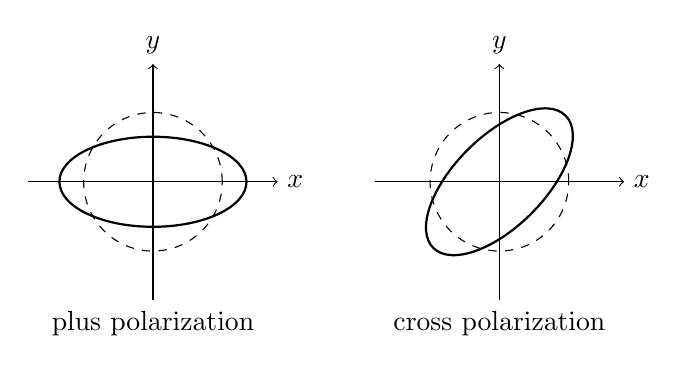
\begin{tikzpicture}[scale=0.88]
\begin{scope}
\draw[->] (-1.8,0) -- (1.8,0) node[right] {$x$};
\draw[->] (0,-1.7) -- (0,1.7) node[above] {$y$};
\draw[dashed] (0,0) circle (1.0);
\draw[thick] (0,0) ellipse (1.35 and 0.65);
\node at (0,-2.05) {plus polarization};
\end{scope}
\begin{scope}[xshift=5.0cm]
\draw[->] (-1.8,0) -- (1.8,0) node[right] {$x$};
\draw[->] (0,-1.7) -- (0,1.7) node[above] {$y$};
\draw[dashed] (0,0) circle (1.0);
\draw[thick,rotate=45] (0,0) ellipse (1.35 and 0.65);
\node at (0,-2.05) {cross polarization};
\end{scope}
\end{tikzpicture}
\caption{Durant une demi-période, une direction transverse s’étire tandis que la direction perpendiculaire se comprime. Une demi-période plus tard, la déformation s’inverse.}
\end{figure}

\section{Des composantes de la métrique à la déformation physique}

Fixons \(z\) et \(t\), puis examinons le plan transverse. Pour une onde purement polarisée plus,
\begin{equation}
 ds_\perp^2
 =(1+h_{xx})\,dx^2+(1-h_{xx})\,dy^2.
 \label{eq:transverse-distance}
\end{equation}
Lorsque \(h_{xx}>0\), un intervalle de coordonnées fixe selon \(x\) a une longueur propre légèrement plus grande, tandis que l’intervalle correspondant selon \(y\) a une longueur légèrement plus petite. Une demi-période plus tard, \(h_{xx}\) change de signe et les rôles s’inversent. Un carré s’étire tour à tour horizontalement et se comprime verticalement, puis se comprime horizontalement et s’étire verticalement. Pour la polarisation croix, la même alternance se produit selon des axes tournés de \(45^\circ\).

Au premier ordre, la longueur initiale \(L\) d’un bras varie de
\begin{equation}
 \frac{\Delta L}{L}\simeq\frac12 h_{ij}n^i n^j,
 \label{eq:fractional-strain}
\end{equation}
où \(\mathbf n\) est dirigé le long du bras. Cette formule traduit la perturbation de la métrique en la déformation relative sans dimension mesurée par un détecteur.

\begin{classroomqa}\audiencequestion{Une règle graduée est maintenue par les forces électromagnétiques et sa longueur au repos ne varie pas simplement avec les coordonnées. Ne faudrait-il pas plutôt représenter des masses d’épreuve librement séparées ?}\lecturerresponse{La distinction est importante. Une tige réelle possède une élasticité : le champ de marée y engendre donc des contraintes internes. Une tige d’acier et une tige de bois réagiront généralement différemment. Des masses d’épreuve suspendues librement évitent cette réponse élastique particulière et révèlent plus directement l’accélération relative. Dans les deux cas, l’onde qui passe ne fait pas que réattribuer des étiquettes aux points. Sa courbure variable dans le temps produit un effet physique.
\lecturetimestamp{00:47:23--00:48:48}}
\end{classroomqa}

La formulation locale précise est celle de la déviation géodésique. Pour des particules voisines en chute libre, séparées par \(\xi^i\),
\begin{equation}
 \frac{d^2\xi^i}{dt^2}
 =-R^i{}_{0j0}\,\xi^j.
 \label{eq:geodesic-deviation}
\end{equation}
Dans une onde faible transverse et sans trace,
\begin{equation}
 R_{0i0j}=-\frac12\ddot h^{\mathrm{TT}}_{ij},
 \label{eq:tidal-curvature}
\end{equation}
la métrique oscillante engendre donc une accélération de marée alternée. C’est pourquoi une onde dépendant du temps ne peut pas être écartée comme un choix statique de règles de mesure. Sa courbure n’est pas nulle.

\begin{classroomqa}\audiencequestion{Qu’est-ce qui peut mesurer la compression et l’étirement si toutes les règles de la région sont affectées ?}\lecturerresponse{Un extensomètre peut enregistrer la contrainte réelle induite dans un corps matériel. Mieux encore, on peut suivre la variation de la distance entre des masses suspendues librement. Une dilatation statique et uniforme pourrait être absorbée par l’appareil de mesure, mais la courbure oscillante engendre une réponse que l’on peut enregistrer.
\lecturetimestamp{00:51:10--00:52:02}}
\end{classroomqa}

\section{Sources et détecteurs}

Les ondes électromagnétiques sont produites par des charges et des courants en mouvement. Les ondes gravitationnelles sont produites par des distributions de masse et d’énergie en mouvement. La conservation de l’énergie et de la quantité de mouvement exclut le rayonnement gravitationnel monopolaire et dipolaire d’un système isolé ; le moment radiatif dominant est donc quadrupolaire. Un système binaire compact fournit précisément le quadrupôle variable nécessaire : deux corps denses orbitent l’un autour de l’autre et émettent des ondes dans le champ lointain.

À proximité du système binaire, l’espace-temps est fortement courbé et le développement linéaire de l’équation~\eqref{eq:weak-split} n’est pas fiable. Au loin, l’onde émise se répartit sur une aire plus grande, son amplitude devient faible et la description linéarisée devient exacte. Pour un observateur situé sur l’axe \(z\) par rapport à la source, l’étirement mesurable se produit dans le plan transverse \(x\)-\(y\).

\begin{classroomqa}\audiencequestion{Dans le dessin, la règle est-elle une règle abstraite de coordonnées ou une règle graduée matérielle ? Et comment une règle variable pourrait-elle mesurer l’effet ?}\lecturerresponse{Il peut s’agir d’un objet matériel, mais ses propriétés entrent alors en jeu. La courbure produit la contrainte de marée ; l’acier et le bois ne se déforment pas nécessairement de la même façon sous son effet. Comparer leurs réponses constitue déjà une mesure. Un détecteur plus simple remplace les tiges par des masses d’épreuve séparées et mesure leur mouvement différentiel.
\lecturetimestamp{00:54:00--00:55:19}}
\end{classroomqa}

Un détecteur résonant est une stratégie possible. Si un système mécanique a une fréquence propre proche de celle de l’onde incidente, celle-ci le met en mouvement de façon cohérente et amplifie sa réponse. Un interféromètre utilise une autre stratégie : les miroirs servent de masses d’épreuve, et les interférences laser permettent de comparer les longueurs effectives de bras perpendiculaires. Une onde polarisée plus allonge un bras tout en raccourcissant l’autre, ce qui constitue précisément le signal différentiel qu’un interféromètre est conçu pour détecter.

\begin{classroomqa}\audiencequestion{Est-ce sur ce principe que repose un détecteur d’ondes gravitationnelles ?}\lecturerresponse{Oui. Une tige rigide se déforme à peine, tandis que des masses terminales librement suspendues peuvent subir une accélération relative. On peut aussi exploiter la résonance, de sorte qu’une faible excitation périodique produise une réponse plus grande. La déformation astrophysique attendue est extraordinairement faible, de l’ordre de \(10^{-21}\) ; concevoir un détecteur consiste donc à transformer ce minuscule mouvement différentiel en un signal mesurable.
\lecturetimestamp{00:55:20--00:57:10}}
\end{classroomqa}

\begin{classroomqa}\audiencequestion{LIGO est-il un exemple de ce type de détecteur ?}\lecturerresponse{Oui. Ses observables fondamentales proviennent de la lumière laser réfléchie entre des miroirs disposés dans des bras perpendiculaires. Une onde gravitationnelle modifie les longueurs optiques relatives et donc la figure d’interférence. À l’époque de cette leçon, l’instrument n’avait pas encore détecté directement d’onde ; la situation historique a ensuite évolué.\editorialnote{150914, la première observation directe, GW2015, a été enregistrée en 2016 et annoncée en }.
\lecturetimestamp{00:57:16--00:58:05}}
\end{classroomqa}

\begin{classroomqa}\audiencequestion{Quelle est la vitesse de propagation déduite de la solution ondulatoire ?}\lecturerresponse{Celle de la lumière. La phase \(k(z-t)\) se déplace d’une unité selon \(z\) pour une unité selon \(t\), et l’équation d’Einstein linéarisée a la même structure de propagation sur le cône de lumière que l’équation des ondes électromagnétiques.
\lecturetimestamp{00:58:07--00:58:16}}
\end{classroomqa}

Les collisions de trous noirs et les systèmes binaires compacts sont des sources particulièrement prometteuses. À proximité de la collision, le champ gravitationnel est fortement non linéaire, et une part substantielle de l’énergie libérée peut être émise sous forme de rayonnement gravitationnel. Lorsque le signal atteint un détecteur distant, son amplitude est suffisamment faible pour que la propagation linéaire des ondes en fournisse une excellente description. Le rayonnement gravitationnel ouvre ainsi une voie d’observation astronomique qui ne dépend pas nécessairement de la lumière émise.

\section{Le pulsar binaire et les preuves indirectes}

Le rayonnement emporte de l’énergie. Si un système binaire émet des ondes gravitationnelles, son énergie orbitale diminue, les corps spiralent lentement l’un vers l’autre et la période orbitale change. Le pulsar binaire fournit une horloge assez précise pour mesurer ce changement. L’évolution orbitale observée est en accord quantitatif avec la perte d’énergie prédite par la relativité générale.

Dans le contexte historique de cette leçon, il s’agissait de la preuve indirecte décisive : aucun détecteur n’avait encore enregistré le passage d’une onde à travers la Terre, mais le système perdait de l’énergie au rythme exigé par le rayonnement gravitationnel. Les ondes étaient déjà observables par leurs effets sur leur source.

\begin{classroomqa}\audiencequestion{Quelle fréquence ou période caractérise le système du pulsar binaire d’origine ? Est-elle de l’ordre de la milliseconde ?}\lecturerresponse{L’échelle de la milliseconde correspond à la rotation du pulsar, pas à l’orbite des deux étoiles. La classe vérifie la valeur et trouve une période orbitale d’environ \(7.75\) heures. Cette distinction est importante : le rayonnement gravitationnel suit le mouvement orbital du système binaire, tandis que les impulsions radio fournissent l’horloge précise qui permet de le suivre.
\lecturetimestamp{01:01:27--01:03:28}}
\end{classroomqa}

\begin{classroomqa}\audiencequestion{De combien le décalage cumulé des temps orbitaux a-t-il varié au cours des décennies d’observation ?}\lecturerresponse{Le décalage cumulé cité est d’environ trente secondes. La variation fractionnaire instantanée est infime, mais des décennies de chronométrage précis des impulsions rendent visible l’effet cumulé.
\lecturetimestamp{01:03:34--01:03:54}}
\end{classroomqa}

\section{Dépendance temporelle, courbure et limites de la linéarité}

\begin{classroomqa}\audiencequestion{Pourquoi choisir le plan transverse \(x\)-\(y\) ? Que se passe-t-il si l’on considère plutôt un plan faisant intervenir \(x\) et \(t\) ?}\lecturerresponse{L’onde elle-même dépend de \(z\) et de \(t\), mais « transverse » désigne les directions spatiales perpendiculaires à sa direction spatiale de propagation. Pour une onde se propageant selon \(z\), on peut choisir les amplitudes physiques de la métrique dans le bloc \(x\)-\(y\). Les autres composantes apparentes sont absentes ou peuvent être éliminées comme de simples ondulations des coordonnées.
\lecturetimestamp{01:02:22--01:03:17}}
\end{classroomqa}

\begin{classroomqa}\audiencequestion{Le temps lui-même oscille-t-il ?}\lecturerresponse{Non. L’onde oscille en fonction du temps. À position spatiale fixe, les composantes \(h_{ij}(z,t)\) varient périodiquement. Le temps est une coordonnée dont dépend le champ, et non un objet qui serait alternativement étiré et comprimé dans cette représentation.
\lecturetimestamp{01:04:00--01:04:18}}
\end{classroomqa}

\begin{classroomqa}\audiencequestion{Si toutes les composantes \(h_{0\mu}\) s’annulent, n’y a-t-il aucune courbure impliquant la direction temporelle ?}\lecturerresponse{Il y en a une. Les composantes spatiales qui subsistent dépendent du temps, et la courbure contient leurs dérivées secondes. Ainsi, des dérivées telles que \(\partial_t^2h_{ij}\) engendrent des composantes \(R_{0i0j}\). L’annulation des composantes de \(h_{\mu\nu}\) comportant un indice temporel n’implique pas que la courbure dépendant du temps soit nulle.
\lecturetimestamp{01:05:15--01:06:09}}
\end{classroomqa}

L’équation d’onde linéaire est apparue parce que l’on a supposé \(h\) petit, et non parce que les artefacts de coordonnées ont été éliminés. Ce sont deux opérations distinctes. La fixation de jauge identifie les degrés de liberté physiques ; la linéarisation néglige les interactions non linéaires.

\begin{classroomqa}\audiencequestion{Les équations d’Einstein sont non linéaires, mais l’équation d’onde obtenue est linéaire. Cette linéarité vient-elle de l’élimination des solutions non physiques ?}\lecturerresponse{Non. Elle vient de l’approximation des faibles amplitudes. On a négligé les termes contenant deux puissances de \(h\). L’élimination des ondulations des coordonnées détermine quelles solutions sont physiques ; elle ne rend pas l’équation linéaire.
\lecturetimestamp{01:06:45--01:07:29}}
\end{classroomqa}

\begin{classroomqa}\audiencequestion{Après résolution de l’équation linéarisée, quelle est l’ampleur de l’erreur par rapport à une solution exacte ?}\lecturerresponse{Les premières corrections négligées sont de l’ordre de \(h^2\). Si \(h\sim10^{-1}\), elles sont de l’ordre de \(10^{-2}\) ; si \(h\sim10^{-3}\), elles sont de l’ordre de \(10^{-6}\). Il faut toujours vérifier après coup un calcul perturbatif afin de s’assurer que le petit paramètre supposé l’était effectivement.
\lecturetimestamp{01:07:35--01:08:31}}
\end{classroomqa}

\begin{classroomqa}\audiencequestion{Quand les termes d’ordre supérieur deviennent importants, l’onde perd-elle son caractère transverse ?}\lecturerresponse{Le caractère transverse essentiel du rayonnement subsiste, mais pas la superposition linéaire. Les ondes fortes interagissent avec le champ gravitationnel transporté par les autres ondes ; au lieu de se traverser sans changer, elles sont diffusées.
\lecturetimestamp{01:08:34--01:09:11}}
\end{classroomqa}

\begin{classroomqa}\audiencequestion{La vitesse d’une onde mécanique dépend de la rigidité et de la masse volumique. Peut-on dire, dans un sens comparable, que l’espace-temps possède une rigidité ?}\lecturerresponse{C’est seulement une analogie. Dans un milieu matériel, la propagation dépend d’une combinaison telle que la rigidité divisée par la masse volumique. Puisque les ondes électromagnétiques et gravitationnelles se propagent à \(c\), le langage de la mécanique classique qualifierait leur milieu d’extraordinairement rigide. La physique moderne n’attribue pas à l’espace-temps un module de Young ordinaire ; le fait invariant est que les équations de champ fixent la propagation à la vitesse de la lumière.
\lecturetimestamp{01:09:12--01:11:10}}
\end{classroomqa}

\section{Autre approche : l’action stationnaire}

La discussion des ondes achevée, il reste le temps d’adopter un dernier point de vue. Le principe de l’action stationnaire est le langage commun de la mécanique classique, de l’électromagnétisme, de la théorie des champs et du Modèle standard. La relativité générale s’inscrit dans cette même structure.

Pour une particule, l’action est une intégrale le long d’une trajectoire. Pour un champ, une histoire associe une valeur du champ \(\phi(x)\) à chaque point de l’espace-temps, et l’action est une intégrale sur l’espace-temps :
\begin{equation}
 S[\phi]
 =\int d^4x\,
 \mathcal L\bigl(\phi,\partial_\mu\phi\bigr).
 \label{eq:field-action}
\end{equation}
Tout \(\phi(x)\) suffisamment régulier constitue une histoire envisageable, de même que tout chemin suffisamment régulier est une trajectoire envisageable pour une particule, mais la plupart ne sont pas des solutions. Les histoires physiques sont les points stationnaires de l’action pour des données aux limites fixées :
\begin{equation}
 \delta S=0.
 \label{eq:stationary-action}
\end{equation}
Pour un champ, la frontière entoure une région de l’espace-temps, au lieu de simplement fixer les deux extrémités d’un chemin. Les équations d’Euler--Lagrange déterminent alors l’interpolation entre les valeurs prescrites sur la frontière.

On peut obtenir les équations de champ d’Einstein exactement de cette manière. Le calcul variationnel est long, mais l’action elle-même est simple. Avant de l’écrire, il nous faut la mesure propre du volume de l’espace-temps.

\section{Pourquoi le déterminant mesure le volume}

Commençons en deux dimensions par une métrique diagonale,
\begin{equation}
 ds^2=g_{xx}\,dx^2+g_{yy}\,dy^2.
\end{equation}
Un rectangle de coordonnées dont les côtés mesurent \(dx\) et \(dy\) a pour longueurs propres
\(\sqrt{g_{xx}}\,dx\) et \(\sqrt{g_{yy}}\,dy\) ; son aire propre est donc
\begin{equation}
 dA
 =\sqrt{g_{xx}g_{yy}}\,dx\,dy.
\end{equation}
Si la composante hors diagonale \(g_{xy}\) est présente, les côtés du rectangle de coordonnées ne sont pas nécessairement orthogonaux. L’aire corrigée vaut
\begin{equation}
 dA
 =\sqrt{g_{xx}g_{yy}-g_{xy}^2}\,dx\,dy
 =\sqrt{\det g}\,dx\,dy.
 \label{eq:area-determinant}
\end{equation}

\begin{figure}[htbp]
\centering
\includegraphics[width=0.84\textwidth]{lecture_10_figure_07.png}
\caption{Généralisation au tableau du petit rectangle de coordonnées à l’élément d’aire propre \(\sqrt{\lvert g\rvert}\,dx\,dy\). Le déterminant tient compte à la fois des longueurs diagonales et du cisaillement dû aux termes hors diagonale.}
\lectureframe{01:21:25}
\end{figure}

La même construction s’applique en toute dimension :
\begin{equation}
 dV_n=\sqrt{|\det g|}\,d^nx.
\end{equation}
Dans l’espace-temps lorentzien, si \(g=\det(g_{\mu\nu})\), l’élément invariant de quatre-volume s’écrit conventionnellement
\begin{equation}
 dV_4=\sqrt{|g|}\,d^4x,
 \label{eq:four-volume}
\end{equation}
ou \(\sqrt{-g}\,d^4x\) avec la convention où la signature comporte davantage de signes plus. Les coordonnées d’une région peuvent changer, mais pas son quatre-volume physique.

La multiplication de cette mesure par un scalaire quelconque \(F(x)\), suivie d’une intégration, produit une quantité invariante par changement de coordonnées :
\begin{equation}
 \int d^4x\,\sqrt{|g|}\,F(x).
 \label{eq:invariant-scalar-integral}
\end{equation}
L’action d’une théorie généralement covariante doit être de cette forme. Sinon, les équations de champ qu’on en déduit pourraient dépendre d’un choix arbitraire de coordonnées.

\section{Action d’Einstein--Hilbert}

En gravitation pure, le champ dynamique est la métrique elle-même. Le scalaire non constant le plus simple que l’on puisse construire à partir de la métrique et de ses deux premières dérivées est la courbure scalaire \(R\). Une constante est également un scalaire ; son coefficient est la constante cosmologique. À des conventions de signe et à des termes de bord près, une normalisation standard de l’action gravitationnelle est
\begin{equation}
 S_{\mathrm{grav}}
 =
 \frac{1}{16\pi G}
 \int d^4x\,\sqrt{|g|}\,(R-2\Lambda).
 \label{eq:einstein-hilbert}
\end{equation}

\begin{figure}[htbp]
\centering
\includegraphics[width=0.84\textwidth]{lecture_10_figure_08.png}
\caption{La représentation de l’histoire du champ et l’action gravitationnelle au tableau. La courbure scalaire fournit la dynamique ; le terme constant est proportionnel au volume de l’espace-temps.}
\lectureframe{01:26:32}
\end{figure}

Le terme proportionnel à \(\Lambda\) est simplement un multiple du volume total de l’espace-temps. L’équation d’onde étudiée précédemment concernait le vide avec \(\Lambda=0\) ; ce terme n’y figurait donc pas.

On ajoute la matière au moyen d’une action de matière,
\begin{equation}
 S=S_{\mathrm{grav}}+S_{\mathrm{matter}}.
\end{equation}
En électromagnétisme, par exemple, la contribution invariante du champ est construite à partir du tenseur antisymétrique \(F_{\mu\nu}\) :
\begin{equation}
 S_{\mathrm{EM}}
 =-\frac14
 \int d^4x\,\sqrt{|g|}\,
 F_{\mu\nu}F^{\mu\nu}.
\end{equation}
La variation de l’action totale par rapport à la métrique inverse définit le tenseur énergie-impulsion et donne
\begin{equation}
 R_{\mu\nu}
 -\frac12 g_{\mu\nu}R
 +\Lambda g_{\mu\nu}
 =8\pi G\,T_{\mu\nu}.
 \label{eq:einstein-from-action}
\end{equation}
L’action compacte contient ainsi les équations de champ complètes. Dans le vide, avec \(\Lambda=0\), elle se réduit à la théorie qui régissait les ondes gravitationnelles étudiées précédemment.

\begin{classroomqa}
\audiencequestion{Où le tenseur énergie-impulsion intervient-il dans le principe variationnel ?}
\lecturerresponse{Il provient des termes supplémentaires qui décrivent la matière et les autres champs. L’énergie électromagnétique, les champs de particules et tout autre contenu matériel contribuent à \(S_{\mathrm{matter}}\). La variation par rapport à la métrique fournit \(T_{\mu\nu}\). L’intégrale qui ne contient que \(\sqrt{|g|}R\) correspond à la théorie gravitationnelle dans le vide.
\lecturetimestamp{01:27:26--01:28:25}}
\end{classroomqa}

La dérivation est simple sur le plan conceptuel, mais pénible sur le plan algébrique. On construit les symboles de Christoffel à partir de la métrique, puis la courbure, que l’on contracte pour former \(R\) ; on multiplie ensuite par le facteur déterminant et l’on fait varier l’expression obtenue. Le professeur plaisante en disant que l’exercice devrait prendre cinq minutes et qu’échouer signifierait échouer au cours, puis admet aussitôt avoir abandonné ce calcul à de nombreuses reprises après y avoir consacré beaucoup plus de temps. Cette plaisanterie souligne un point sérieux : des principes concis n’impliquent pas nécessairement des calculs en composantes courts.

\begin{classroomqa}
\audiencequestion{La variation complète est-elle généralement écrite en toutes lettres dans un ouvrage de relativité ?}
\lecturerresponse{Cela peut être le cas, mais le calcul remplit alors des pages. Un long calcul ne devient éclairant que si l’on en suit assez d’étapes pour comprendre pourquoi la suivante s’ensuit ; lire passivement ligne après ligne permet rarement d’acquérir cette compréhension. Les outils modernes de calcul formel et numérique peuvent prendre en charge une grande partie des opérations, mais ils ne remplacent pas le principe directeur.
\lecturetimestamp{01:31:10--01:34:16}}
\end{classroomqa}

Il existe deux approches traditionnelles de ce type de calcul. On peut développer une intuition géométrique assez solide pour discerner quelles combinaisons tensorielles sont possibles, ou bien mener les calculs algébriques avec soin. La plupart des travaux combinent ces deux approches, souvent en confiant à un ordinateur les contractions les plus longues. Le cours a délibérément mis l’accent sur les principes qui restent valables quelle que soit l’approche choisie.

\begin{classroomqa}
\audiencequestion{Rétrospectivement, l’action semble très bien motivée. Pourquoi le passage de la relativité restreinte à la relativité générale a-t-il pris tant d’années à Einstein, et visait-il la théorie finale dès le début ?}
\lecturerresponse{Une fois la géométrie nécessaire connue, le résultat final paraît plus simple. À l’époque, la géométrie différentielle nécessaire était peu familière à la plupart des physiciens, et Einstein a dû l’apprendre et l’adapter avec l’aide de mathématiciens, notamment Marcel Grossmann. Construire les concepts d’espace-temps courbe et trouver l’équation de champ correcte en une dizaine d’années ne relève pas d’un travail lent. Les premiers articles et les articles finaux méritent d’être lus précisément parce qu’ils montrent tout ce qu’il a fallu inventer en chemin.
\lecturetimestamp{01:34:20--01:35:59}}
\end{classroomqa}

Le trimestre s’achève donc sur deux formulations complémentaires d’une même théorie. L’équation de champ indique comment la courbure réagit localement au tenseur énergie-impulsion. Le principe variationnel dit que l’histoire entière de l’espace-temps est un point stationnaire d’une fonctionnelle invariante. Dans la région lointaine où le champ est faible, les deux descriptions se réduisent à des ondes transversales qui transportent une courbure réelle à la vitesse de la lumière.